\documentclass[11pt]{report}
\usepackage[pdftex]{graphicx}
\usepackage{henrian-more}
\usepackage{amsmath}
\usepackage{subfig}
\usepackage{booktabs}
\usepackage{rotating}
\usepackage{float}

\makeHeaders{Machine Learning: Homework 5}

\begin{document}

\begin{itemize}
  \item \textbf{Email}: chrisbrown@utexas.edu
  \item \textbf{EID}: chb595
\end{itemize}

\section{Hyperbolic tangent}
We want to show that:
\[ \text{tanh}(x) \overset{?}{=} 2g(2x) - 1 \]
where:
\[ g(x) = \frac{1}{1 + e^{-x}} \]
First, multiply g(x) out of the equation:
\[ \text{tanh}(x) \overset{?}{=} 2\left(\frac{1}{1 + e^{-2x}}\right) - 1 =
  \frac{2}{1 + e^{-2x}} - 1 =
  \frac{2}{1 + e^{-2x}} - \frac{1 + e^{-2x}}{1 + e^{-2x}} =
  \frac{2 - (1 + e^{-2x})}{1 + e^{-2x}} =
  \frac{1 - e^{-2x}}{1 + e^{-2x}}
\]

\medskip\noindent
Second, by definition, and simple algebra:
\[ \text{tanh}(x) =
  \frac{\text{sinh}(x)}{\text{cosh}(x)} =
  \frac{\frac{e^{x} - e^{-x}}{2}}{\frac{e^{x} + e^{-x}}{2}} =
  \frac{e^{x} - e^{-x}}{e^{x} + e^{-x}} = 
  \frac{\frac{1}{e^{-x}} - e^{-x}}{\frac{1}{e^{-x}} + e^{-x}} = 
  \frac{e^{-x}}{e^{-x}} \cdot \frac{\left(\frac{1}{e^{-x}} - e^{-x}\right)}{\left(\frac{1}{e^{-x}} + e^{-x}\right)} =
  \frac{1 - e^{-2x}}{1 + e^{-2x}}
\]

\medskip\noindent
By merging these, it's clear that:
\[ \frac{1 - e^{-2x}}{1 + e^{-2x}} \overset{\checkmark}{=} \frac{1 - e^{-2x}}{1 + e^{-2x}} \]

% \begin{figure}[H]
%   \centering
%   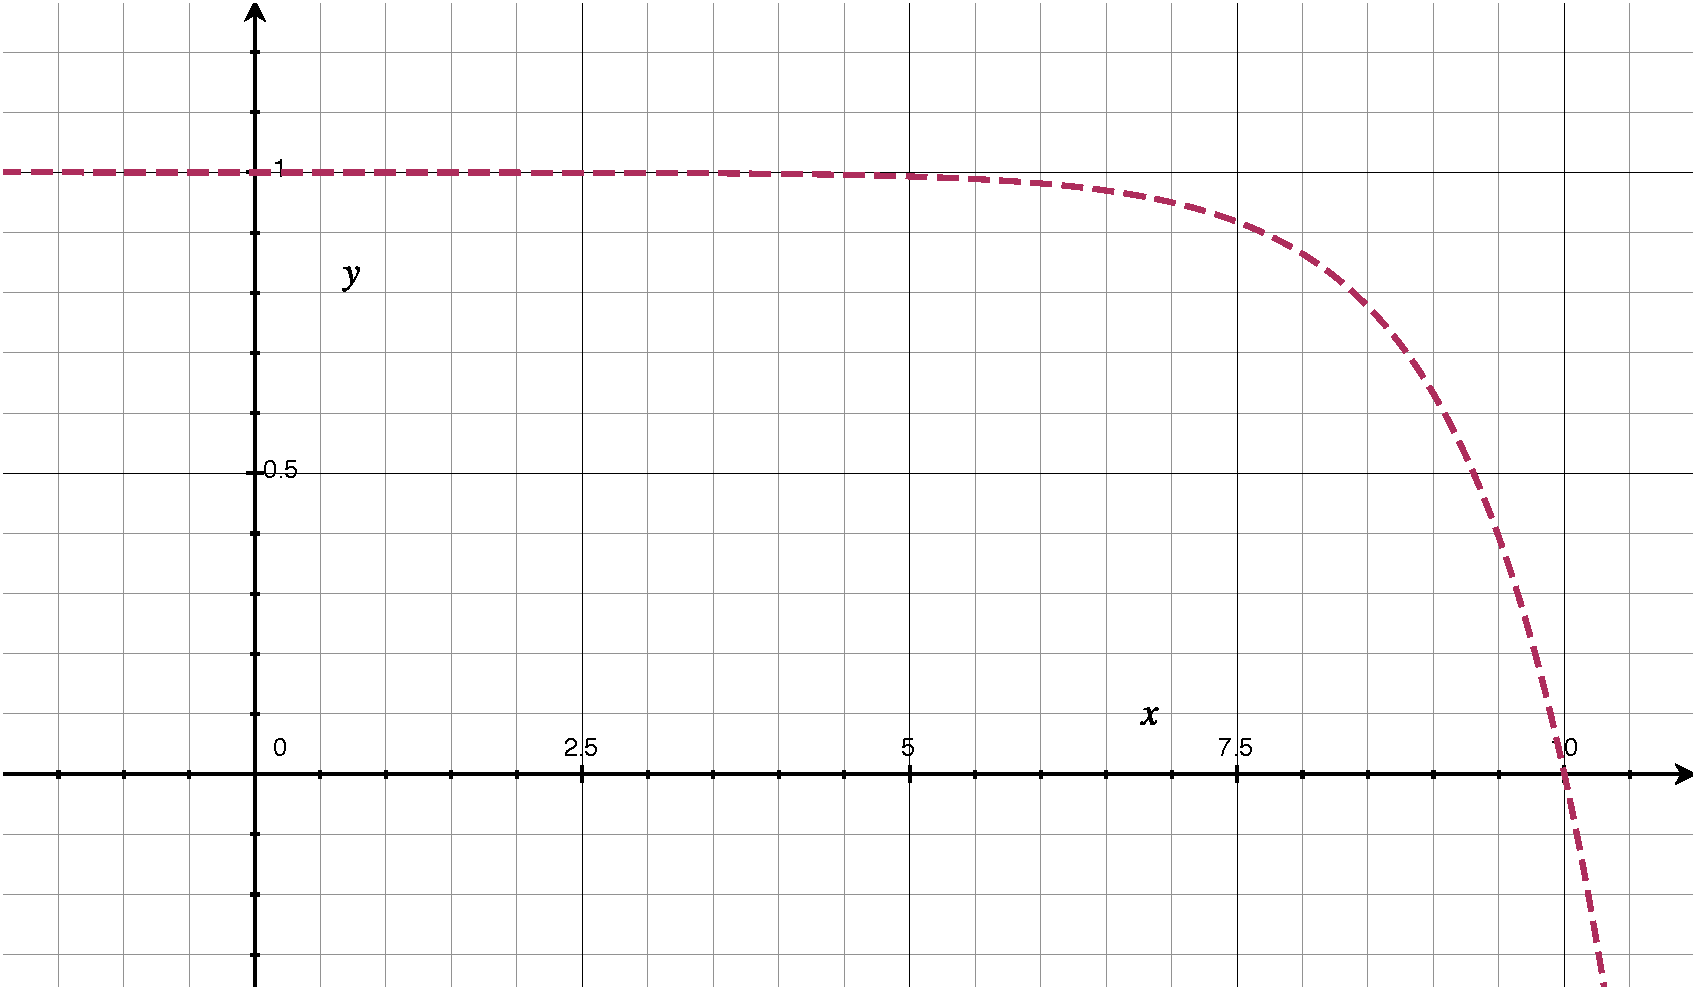
\includegraphics[width=0.9\textwidth]{u-power.pdf}
%   \caption{Power applied at time $t$, for a race 10 seconds long.}
%   \label{fig:power}
% \end{figure}

\bigskip\noindent
We can rewrite g(x) in terms of tanh(x), given that we know the equality:
\[\frac{\text{tanh}(\frac{x}{2}) + 1}{2} = g(x)\]
where $g(x)$ is just equation we were using originally.

\smallskip\noindent
And then instead of differentiating \(\frac{1}{1 + e^{-x}}\), we could differentiate
\[
  \frac{1}{2}\left(\text{tanh}(\frac{x}{2})\right) + \frac{1}{2}
\]
and achieve the same result, which may be easier or more useful, since
\[ \frac{d}{dx} \text{tanh}(x) = 1 - \text{tanh}^2(x) \]

\section{XOR}

I did not find the class suitably equipped me to answer this question, so I resorted to R. Rojas's \emph{Neural Networks}, which outlined the following solution. If this answer is not what the question is asking for, the shortcoming is only because I cannot recall hand-designing any neural networks in class.

The XOR problem itself is not linearly separable. However, we can split the inputs into sub-layers that are linearly separable, and then combine those.

\begin{center}
  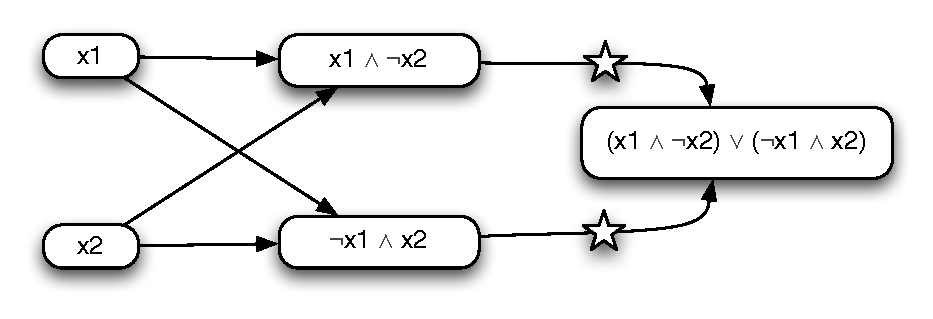
\includegraphics[width=0.8\textwidth]{xor.pdf}
\end{center}
In the network above, the stars designate points at which we can solve two linearly separable problems:

\hfil
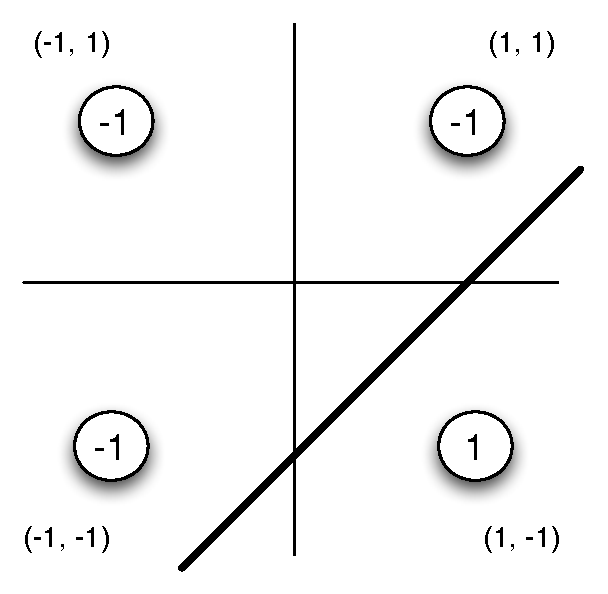
\includegraphics[width=0.3\textwidth]{xor-1st.pdf}
\hfil
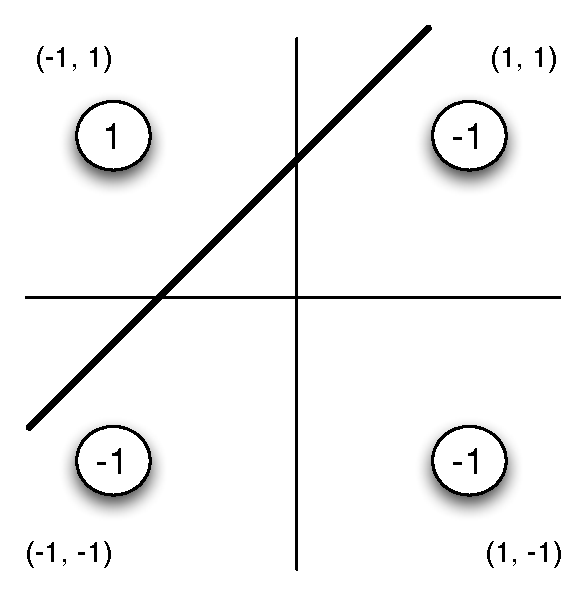
\includegraphics[width=0.3\textwidth]{xor-2nd.pdf}
\hfil

\medskip\noindent
And then, we simply find the disjunction of these two results to achieve the decision/result we desired in the initial problem.

\section{Separation of Two Classes}

We never used the $\rho$ variable name in class, so I presume that for this question, it refers to half the separation distance between two classes of variables, since \texttt{Week6\_SVM.pdf} points out that the true separating distance is \(\frac{2}{||\mathbf{w}_0||}\). Of course, the margin and the separating distance are not the same thing; the separating distance is twice the margin, by definition. Why the class notes use $\mathbf{w}_0$, whereas Bishop does not, I don't know. Presumably $\mathbf{w}_0$ is equivalent to $\mathbf{w}$, as in Bishop. I found this especially confusing, since Bishop uses $w_0$ for the bias vector, whereas the class notes use $b$.

Heeding the emailed instructions (``2012\_spring\_53190\_CS\_391L: hw5 typo''), notation will follow the Bishop style.

We define our separation surface as a set of vectors $\mathbf{x}$, such that \(\mathbf{w}^\text{T}\mathbf{x} + w_0 = 0\).
$\mathbf{w}$ is defined as the weights by which we multiply/collapse a vector (and then add some offset) to determine what class it lies in. That is, each value of $\mathbf{w}$ scales each dimension of some vector a certain way. The bias/threshold $w_0$ is the re-centering adjustment that shifts the $\mathbf{w}$ surface (which intersects the origin) perpendicularly into some other location.

The linear discrimination function \(y(\mathbf{x}) = \mathbf{w}^\text{T}\mathbf{x} + w_0\) returns a scalar number which separates the two classes at $0$. However, usually, the support vectors (vectors closest to the separating surface) are not directly on top of the line, but some distance away. Note that since the separating surface is just a dividing hyperplane, it doesn't actually matter what its magnitude is, for the purposes of orienting it (and positioning it via $w_0$) within the vector-space. It could be defined by a unit vector. The magnitude, then, can be defined as we like, and we have defined it such that the distance from the hyperplane to the closest support vector is precisely $\frac{1}{||\mathbf{x}||}$.

We can also show this more mathematically. The distance from a hyperplane/surface parameterized by $\mathbf{w}$ and $w_0$ for some point $\mathbf{x}$ is shown by Bishop to be $\frac{y(\mathbf{x})}{||\mathbf{w}||}$. Expanded, this is
\[
  \frac{\mathbf{w}^\text{T}\mathbf{x} + w_0}{||\mathbf{w}||}
\]
Now let's pick out two vectors, $\mathbf{x}_{-1}$ and $\mathbf{x}_{+1}$, both of which are subscripted by the class they belong to. We know we have at least these two vectors, both support vectors, though we may have more. We can define the magnitude of $\mathbf{w}$ however we want, as was explained in the last paragraph. And we have decided that $y(\mathbf{x})$ for the support vectors of the positive class should give us $+1$, and $-1$ for the negative class. So:
\begin{align*}
  \mathbf{w}^\text{T}\mathbf{x_{-1}} + w_0 = -1
  & &
  \text{and}
  & &
  \mathbf{w}^\text{T}\mathbf{x_{+1}} + w_0 = +1
\end{align*}
And after rearranging:
\begin{align*}
  \mathbf{w}^\text{T}\mathbf{x_{-1}} = -1 - w_0
  & &
  \text{and}
  & &
  \mathbf{w}^\text{T}\mathbf{x_{+1}} = 1 - w_0
\end{align*}
Projected onto a line perpendicular to the separating surface, the distance between these two vectors should be precisely equal to $\frac{2}{||\mathbf{w}||}$.

A vector $\mathbf{a}$ projected onto a vector $\mathbf{b}$ has a magnitude of $\mathbf{a}^\text{T}\mathbf{b}$, which we can then align in the same direction as $\mathbf{b}$ by multiplying by $\frac{\mathbf{b}}{||\mathbf{b}||}$. But since we only want to compare the distance between $\mathbf{x_{-1}}$ and $\mathbf{x_{+1}}$ along the same direction (namely, $\mathbf{w}$), we can just compare their magnitudes along $\mathbf{w}$.
\[
  \mathbf{x_{+1}}^\text{T}\mathbf{w} - \mathbf{x_{-1}}^\text{T}\mathbf{w} \overset{?}{=} 2
\]
Of course, when $\mathbf{a}$ and $\mathbf{b}$ are both column vectors, $\mathbf{a}^\text{T}\mathbf{b}$ = $\mathbf{b}^\text{T}\mathbf{a}$, so we can just substitute in our values from earlier:
\[
  1 - w_0 - (-1 - w_0) = 1 - w_0 + 1 + w_0 = 2 \overset{\checkmark}{=} 2
\]
And so, it should be clear that:
\[
  \frac{\mathbf{x_{+1}}^\text{T}\mathbf{w}}{||\mathbf{w}||} - \frac{\mathbf{x_{-1}}^\text{T}\mathbf{w}}{||\mathbf{w}||} \overset{\checkmark}{=} \frac{2}{||\mathbf{w}||}
\]

\section{Bishop 7.4}

Bishop has already shown that we can define the \emph{margin} (which is not the separating distance) as
\[ \rho = \frac{1}{||\mathbf{w}||} \]
From which we can easily derive
\[ \frac{1}{\rho} = ||\mathbf{w}|| \]
And
\[ \frac{1}{\rho^2} = ||\mathbf{w}||^2 = \mathbf{w}^\text{T}\mathbf{w} \]
So we want to show that 
\[ \mathbf{w}^\text{T}\mathbf{w} \overset{?}{=} \sum^N_{n=1} a_n \]
where all the $a_n$ values are positive (7.11) and \( \sum^N_{n=1} a_nt_n = 0 \), where $t_n \in \{-1, +1\}$ (7.12).

\medskip\noindent
At the solution/maximum, \(L(\mathbf{w}, b, \mathbf{a}) = \frac{1}{2}||\mathbf{w}||^2\) (7.7), which of course is the same thing as \(L(\mathbf{w}, b, \mathbf{a}) = \frac{1}{2}\mathbf{w}^\text{T}\mathbf{w}\).

We can take the dual representation of the maximum from (7.10):
\[\tilde{L}(\mathbf{a}) = \sum^N_{n=1} a_n - \frac{1}{2}\dots \]
and substitute just $\mathbf{w}$ back into the equation, where $\mathbf{w} = \sum^N_{n=1} a_nt_n\Phi(x_n)$ from (7.8), which produces:
\[ \tilde{L}(\mathbf{a}) = \sum^N_{n=1} a_n - \frac{1}{2} \mathbf{w}^\text{T}\mathbf{w} \]

Combining $\tilde{L}(\mathbf{a})$ and $L(\mathbf{w}, b, \mathbf{a})$, we have:
\[
  \frac{1}{2}\mathbf{w}^\text{T}\mathbf{w} = \sum^N_{n=1} a_n - \frac{1}{2} \mathbf{w}^\text{T}\mathbf{w}
\]
Adding both $\frac{1}{2}\mathbf{w}^\text{T}\mathbf{w}$ to both sides, we achieve precisely what we wanted to prove:
\[ \mathbf{w}^\text{T}\mathbf{w} \overset{\checkmark}{=} \sum^N_{n=1} a_n \]

\section{Bishop 7.5}

\[
  \frac{1}{\rho^2} \overset{?}{=} 2\tilde{L}(\mathbf{a})
\]
We can then use the derivation of (7.10) that substituted back in $\textbf{w}$, to replace $\tilde{L}(\mathbf{a})$ on the right side of the equation.
\[
  \frac{1}{\rho^2} \overset{?}{=} 2\sum^N_{n=1} a_n - \textbf{w}^\text{T}\textbf{w}
\]
Then, using what we proved in 7.4:
\[
  \frac{1}{\rho^2} \overset{?}{=} 2\textbf{w}^\text{T}\textbf{w} - \textbf{w}^\text{T}\textbf{w}
\]
Which reduces to:
\[
  \frac{1}{\rho^2} \overset{\checkmark}{=} \textbf{w}^\text{T}\textbf{w}
\]
Which is one of the equations we started with in 7.4, above.

\medskip\noindent
I'm afraid I don't see how the second part of Bishop's Exercise 7.5 (7.125) is any different from the equation we just ended up with, or how we could prove the equation in (7.125) except by retracing our steps and ``proving'' it circularly from the result we just achieved.


\section{Kernel Unitary Invariance}

We want to show that 
\[
  K(\mathbf{x}, \mathbf{x_i}) \overset{?}{=} K(Q\mathbf{x}, Q\mathbf{x_i})
\]
We use the definition of $K$ to expand both sides:
\[
  (1 + \mathbf{x}^\text{T}\mathbf{x_i})^p \overset{?}{=}
  (1 + (Q\mathbf{x})^\text{T}Q\mathbf{x_i})^p
\]
And rearrange the right side:
\[
  (1 + \mathbf{x}^\text{T}\mathbf{x_i})^p \overset{?}{=}
  (1 + \mathbf{x}^\text{T}Q^\text{T}Q\mathbf{x_i})^p
\]
Since $Q$ is unitary, $Q^{-1}$ = $Q^T$ and $Q^{-1}Q = I$:
\[
  (1 + \mathbf{x}^\text{T}\mathbf{x_i})^p \overset{?}{=}
  (1 + \mathbf{x}^\text{T}I\mathbf{x_i})^p
\]
And the $I$ just falls out:
\[
  (1 + \mathbf{x}^\text{T}\mathbf{x_i})^p \overset{\checkmark}{=}
  (1 + \mathbf{x}^\text{T}\mathbf{x_i})^p
\]



\section{The Kernel Trick}

When a classification of vectors is linearly inseparable in its original state, it can often by projected into another vector-space, and linearly separated there.
Kernels are used to do this---to boost vectors from one projection into another of much higher dimensionality. This can involve a \emph{lot} of multiplication, producing a lot of extraneous values.
The `kernel trick' is an optimization that allows us to take a shortcut through all the multiplications, and operate on a sort of halfway-projection.

% When we have a kernal-applicable vectorspace, by definition our kernal function depends exclusively 
% The Kernel Trick is a way of 
For example, if we have a kernel $K(x,y) = (1 + x^\text{T}y)^2$, after all the arithmetic to expand the kernel, we end up with what we can reduce to a dot product for some function $\Phi$, i.e. $\Phi(x) \cdot \Phi(y)$.
The presumption/trick is that since we only need the dot product, we can combine the operations of the remapping ($\Phi$) and the dot project into one mathematical operation, discarding/disregarding what is produced in the middle of these two steps. Effectively, by defining a $\Psi(x, y) = \Phi(x) \cdot \Phi(y)$, we can state that $\Psi(x, y) = K(x, y)$ and declare that we've optimized out the $\Phi$-remapping step.

Note that if our kernel does not reduce to a dot product between the same linear transform of the original two vectors (all of our kernels take two vectors, and return a scalar value), we cannot use the ``kernel trick.''



% Now we can refactor the left side:
% \[ (\mathbf{x_{+1}} - \mathbf{x_{-1}})^\text{T}\mathbf{w} \overset{?}{=} \frac{2}{||\mathbf{w}||} \]
% And expand the right:
% \[
  % (\mathbf{x_{+1}}^\text{T} - \mathbf{x_{-1}}^\text{T})\mathbf{w} \overset{?}{=} \frac{2}{||\mathbf{w}||}
% \]


% For $\mathbf{x_{-1}}$, this just gives us 
 % \mathbf{w}



\end{document}


